
\section{Architecture Integration}

\subsection{Model Support}

\begin{table}[H]
\centering
\small
\begin{tabular}{lllllll}
\toprule
\textbf{Model} & \textbf{Layers} & \textbf{$d$} & \textbf{$H$} & \textbf{$H_{kv}$} & \textbf{Nested?} & \textbf{Conv1D?} \\
\midrule
DistilBERT-base & 6 & 768 & 12 & 12 & No & No \\
RoBERTa-base & 12 & 768 & 12 & 12 & Yes & No \\
GPT-2 & 12 & 768 & 12 & 12 & No & Yes \\
Qwen3.5-0.8B & 24 & 1024 & 8 & 2 & No & No \\
\bottomrule
\end{tabular}
\end{table}

\subsection{DistilBERT (Flat)}

\begin{lstlisting}
distilbert.transformer.layer.0.attention
+-- q\_lin  (Linear 768 $\to$ 768)
+-- k\_lin  (Linear 768 $\to$ 768)
+-- v\_lin  (Linear 768 $\to$ 768)
+-- out\_lin (Linear 768 $\to$ 768)
\end{lstlisting}

All four are \texttt{nn.Linear}. Direct factorization.

\texttt{is\_nested\_encoder = False} because \texttt{out\_lin} is inside the attention.

\subsection{RoBERTa (Nested)}

\begin{lstlisting}
roberta.encoder.layer.0.attention
+-- self
|   +-- query
|   +-- key
|   +-- value
+-- output
    +-- dense  # $\leftarrow$ outside
\end{lstlisting}

\textbf{Critical:} \texttt{output.dense} sits outside. SVD-LLM V2 sets 
\texttt{is\_nested\_encoder = True} and skips \texttt{out\_proj}.

\textbf{Detection.} In \texttt{copy\_weights}:

\begin{lstlisting}
if hasattr(old\_attn, "self") and hasattr(old\_attn, "output"):
    src = old\_attn.self
    if hasattr(old\_attn.output, "dense"):
        w\_o, b\_o = \_unpack\_weight\_bias(old\_attn.output.dense)
    # Note: even though we extract W\_O, we set is\_nested\_encoder=True
    # so it will NOT be used in forward.
\end{lstlisting}

Wait -- SVD-LLM V2 \textbf{does} extract \texttt{W\_O} from the outer layer but **skips 
it** in forward if nested. This may seem redundant but keeps the code 
uniform. In our experiments, this extraction is only used to validate 
weight availability; the actual out projection is applied by the outer 
\texttt{BertSelfOutput.dense}.

\subsection{GPT-2 (Causal Conv1D)}

\begin{lstlisting}
transformer.h.0.attn
+-- c\_attn  (Conv1D 768 $\to$ 2304)   # fused Q, K, V
+-- c\_proj  (Conv1D 768 $\to$ 768)
\end{lstlisting}

\textbf{Split c\_attn:}

\begin{lstlisting}
c\_attn\_w, c\_attn\_b = \_unpack\_weight\_bias(src.c\_attn)
split\_size = c\_attn\_w.size(0) // 3
w\_q = c\_attn\_w[:split\_size, :]
w\_k = c\_attn\_w[split\_size : 2 * split\_size, :]
w\_v = c\_attn\_w[2 * split\_size :, :]
\end{lstlisting}

\textbf{Conv1D transposition:} \texttt{\_unpack\_weight\_bias} handles this automatically:

\begin{lstlisting}
if "Conv1D" in type(module).\_\_name\_\_ or hasattr(module, "nf"):
    w = w.t()
\end{lstlisting}

\texttt{is\_nested\_encoder = False} because \texttt{c\_proj} is inside the attention.

\subsection{Qwen3.5 (GQA + RoPE)}

\begin{lstlisting}
model.layers.0.self\_attn
+-- q\_proj  (Linear 1024 $\to$ 2048)   # H * d\_h
+-- k\_proj  (Linear 1024 $\to$ 512)    # H\_kv * d\_h
+-- v\_proj  (Linear 1024 $\to$ 512)
+-- o\_proj  (Linear 2048 $\to$ 1024)
\end{lstlisting}

\textbf{GQA pooling.} When source \texttt{W\_K} has more rows than \texttt{self.kv\_head\_size}:

\begin{lstlisting}
rep = w\_k.shape[0] // self.kv\_head\_size
w\_k\_pooled = (
    w\_k.view(self.num\_kv\_heads, rep, self.head\_dim, -1)
    .mean(dim=1)
    .view(self.kv\_head\_size, -1)
)
\end{lstlisting}

\textbf{RoPE handling.} Qwen passes \texttt{position\_embeddings} in kwargs. SVD-LLM V2 
applies RoPE after projection.

\texttt{is\_nested\_encoder = False}.

\subsection{Nested Encoder Bypass}

When \texttt{is\_nested\_encoder = True}:

\begin{lstlisting}
context = torch.matmul(probs, V).transpose(1, 2).contiguous().view(...)

if self.is\_nested\_encoder:
    out = context       # $\leftarrow$ No out\_proj
else:
    out = self.\_project(context, ...)   # $\leftarrow$ out\_proj applied
\end{lstlisting}

The outer \texttt{BertSelfOutput.dense} then applies the projection.

\subsection{Injection Protocol}

SVD-LLM V2's injection hook has three safety layers:

\subsubsection{Pre-Test}

\begin{lstlisting}
test\_src = layer\_list[0].attention
try:
    test\_module = SVDLLMV2Attention(cfg, old\_attn=test\_src, ...)
except Exception as e:
    logger.warning(f"Pre-test failed: {e}")
    return None
\end{lstlisting}

\subsubsection{Double-Injection Guard}

\begin{lstlisting}
if isinstance(src, SVDLLMV2Attention) or "SVDLLMV2" in src.\_\_class\_\_.\_\_name\_\_:
    return None
\end{lstlisting}

\subsubsection{Frobenius Validation}

\begin{lstlisting}
for name, w in [("w\_q", w\_q), ("w\_k", w\_k), ("w\_v", w\_v)]:
    if torch.norm(w.float(), p="fro").item() \textless{} 1e-4:
        raise RuntimeError(f"Near-zero norm on {name}")
\end{lstlisting}

\subsection{Failure Modes and Fallbacks}

\begin{table}[H]
\centering
\small
\begin{tabular}{lll}
\toprule
\textbf{Failure} & \textbf{Detection} & \textbf{Response} \\
\midrule
Missing weights & Pre-test or \texttt{copy\_weights} raises & Abort injection \\
Near-zero Frobenius & Norm check \textless{} 1e-4 & Raise \\
Shape mismatch & Padding in \texttt{\_decompose\_and\_set} & Warn \\
Double injection & Class name guard & Skip \\
Cross-attention & Not supported & Not implemented \\
\bottomrule
\end{tabular}
\end{table}

\subsection{Registry}

\begin{lstlisting}
@ATTENTION\_REGISTRY.register("svd\_llm\_v2")
@ATTENTION\_REGISTRY.register("svd\_llm\_v2\_attention")
class SVDLLMV2Attention(BaseAttention):
    ...

@ATTENTION\_REGISTRY.register("svd\_llm\_v2\_inject")
@ATTENTION\_REGISTRY.register("inject\_svd\_llm\_v2")
def inject\_svd\_llm\_v2(...):
    ...
\end{lstlisting}

\subsection{Interaction with LoRA Recovery Pipeline}

SVD-LLM V2 integrates cleanly with the framework's LoRA recovery:

\begin{enumerate}
\item \textbf{Inject} SVD-LLM V2 $\to$ explicit factor buffers, frozen.
\item \textbf{LoRA adapters} per projection (q/k/v/out) are trainable.
\item \textbf{Recovery fine-tuning} trains only LoRA parameters.
\item \textbf{Evaluation} uses the fine-tuned model.

\end{enumerate}
The framework's \texttt{get\_recovery\_params} finds \texttt{\textit{\_lora\_A}, \texttt{}\_lora\_B} 
parameters by naming convention.

\subsection{Comparison with Companion Methods}

\begin{lstlisting}

---
\end{lstlisting}

\begin{figure}[H]
\centering
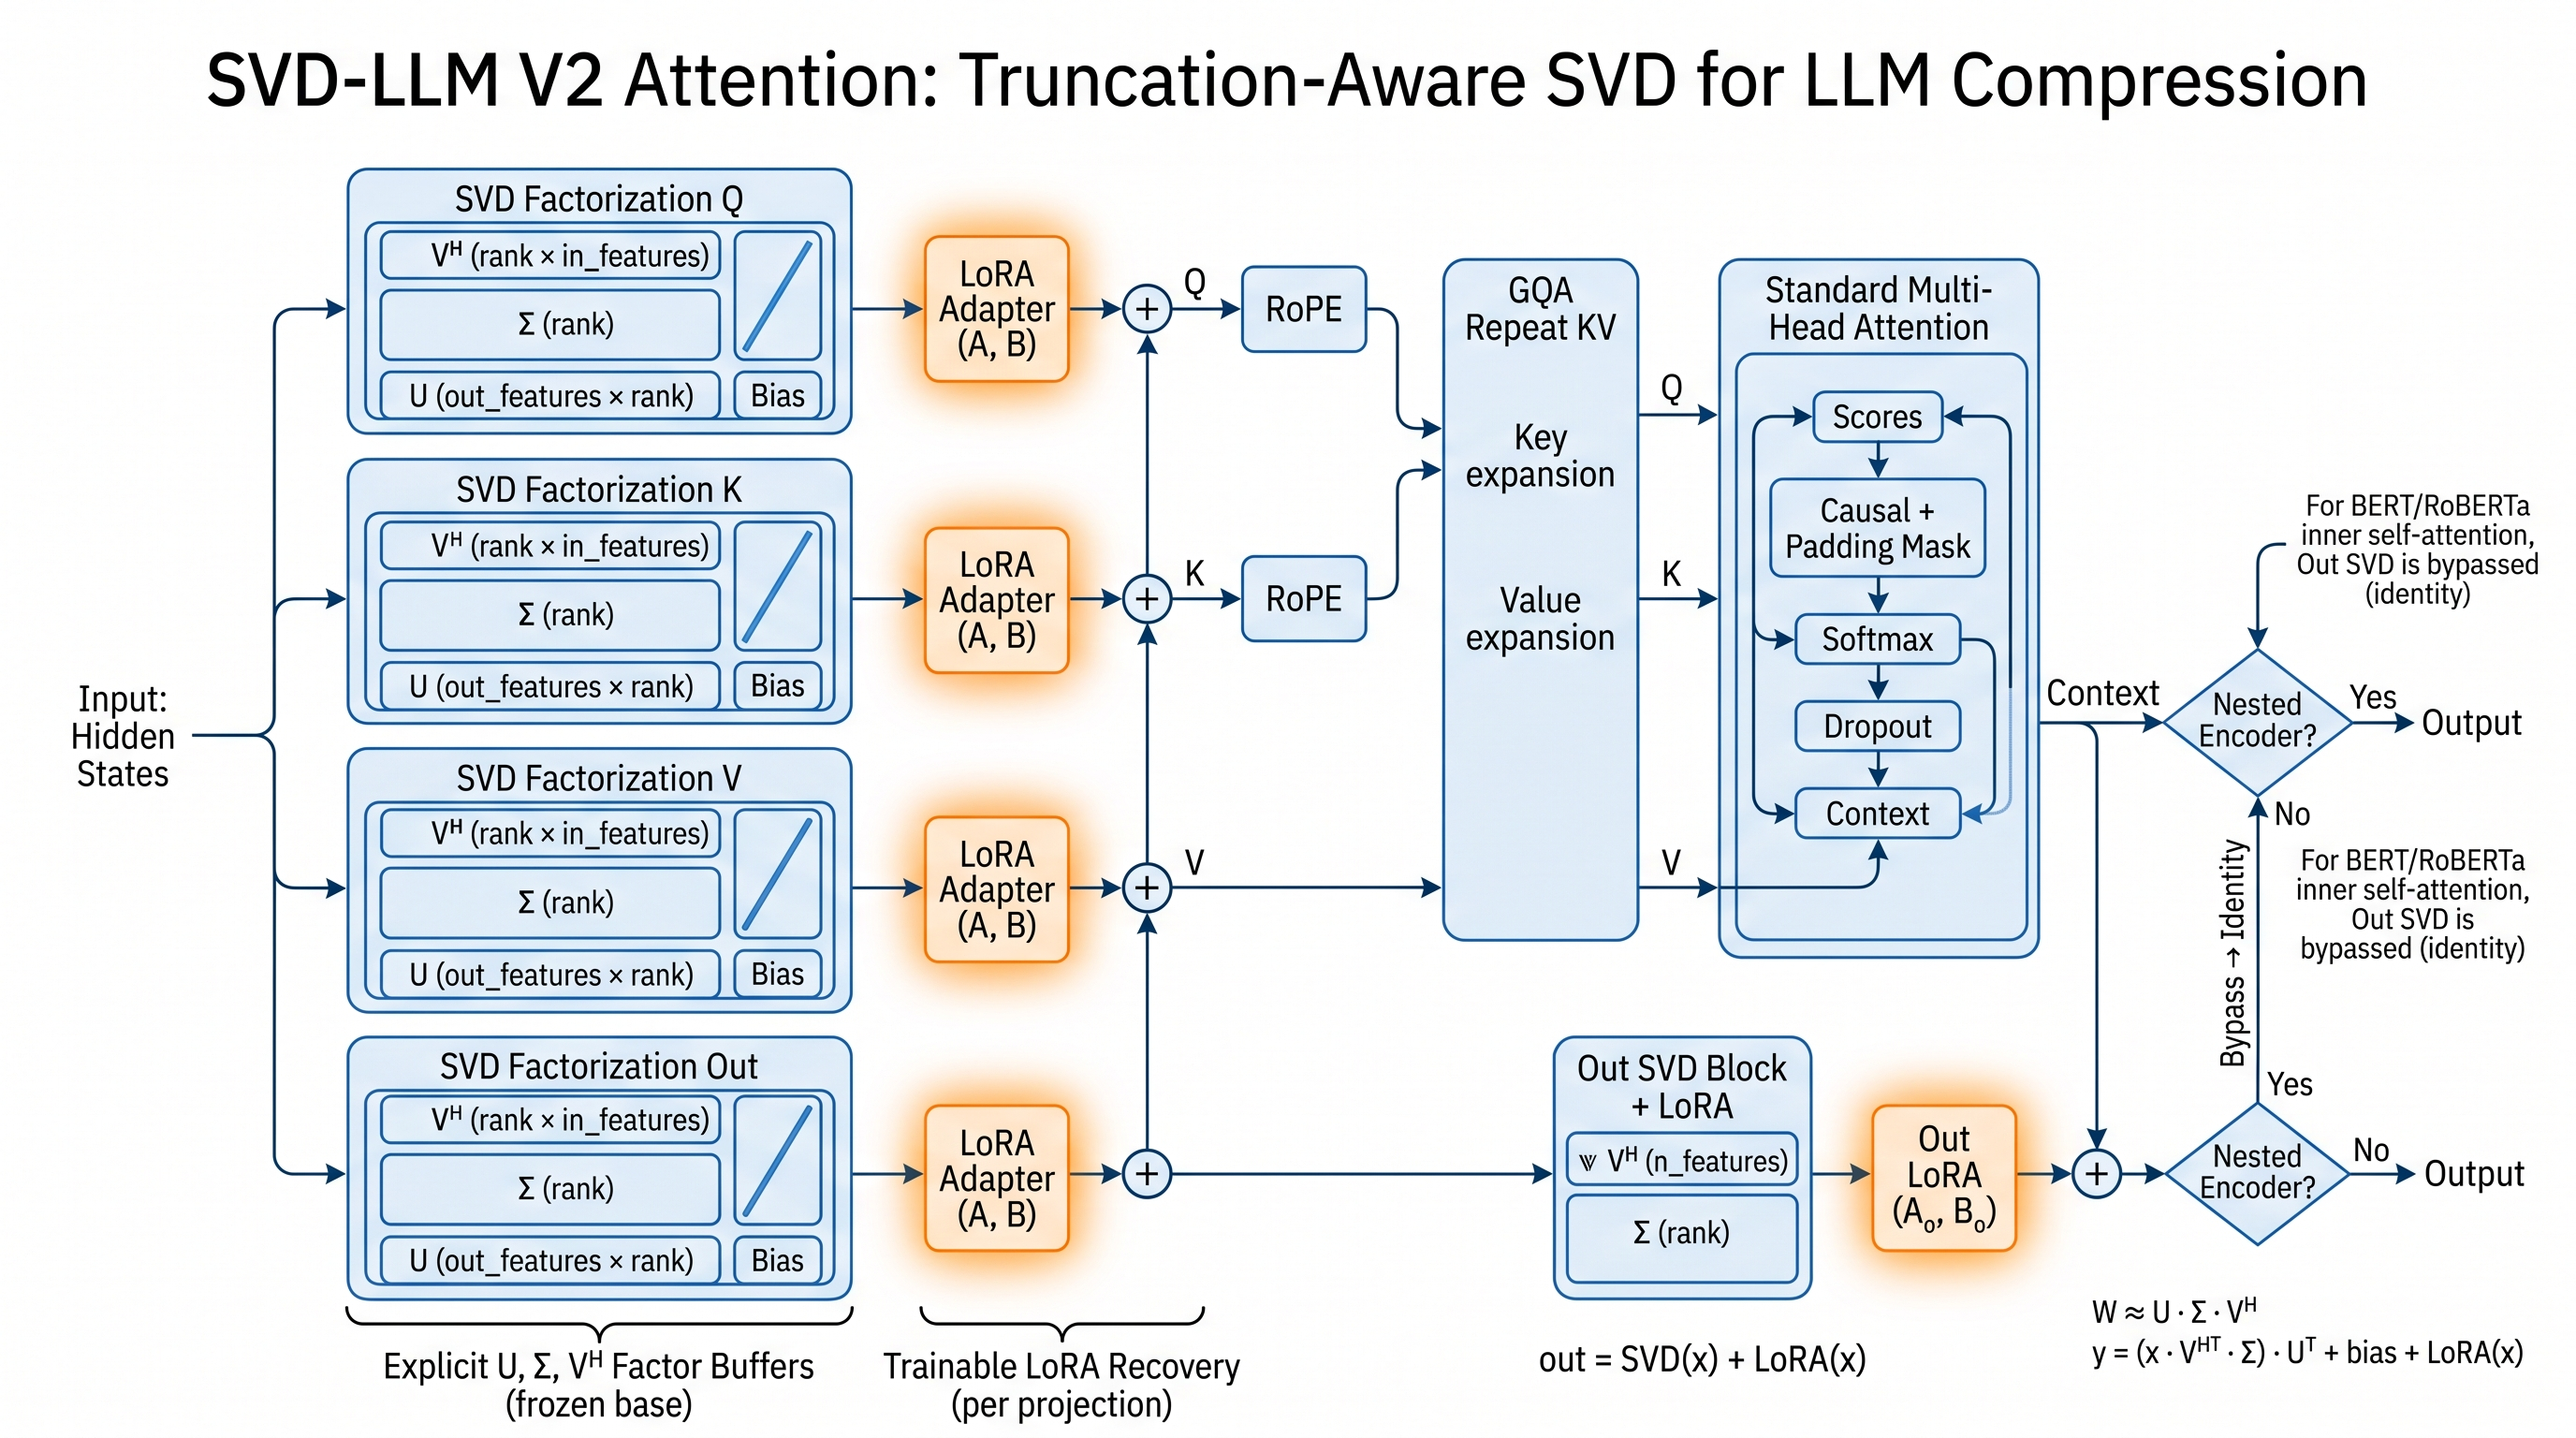
\includegraphics[width=\linewidth]{figures/architecture.jpeg}
\caption{High-level architectural diagram of svd\_llm\_v2\_attention.}
\label{fig:arch_svd-llm-v2-attention}
\end{figure}

